\documentclass[]{article}
\usepackage{lmodern}
\usepackage{amssymb,amsmath}
\usepackage{ifxetex,ifluatex}
\usepackage{fixltx2e} % provides \textsubscript
\ifnum 0\ifxetex 1\fi\ifluatex 1\fi=0 % if pdftex
  \usepackage[T1]{fontenc}
  \usepackage[utf8]{inputenc}
\else % if luatex or xelatex
  \ifxetex
    \usepackage{mathspec}
  \else
    \usepackage{fontspec}
  \fi
  \defaultfontfeatures{Ligatures=TeX,Scale=MatchLowercase}
\fi
% use upquote if available, for straight quotes in verbatim environments
\IfFileExists{upquote.sty}{\usepackage{upquote}}{}
% use microtype if available
\IfFileExists{microtype.sty}{%
\usepackage{microtype}
\UseMicrotypeSet[protrusion]{basicmath} % disable protrusion for tt fonts
}{}
\usepackage[margin=1in]{geometry}
\usepackage{hyperref}
\hypersetup{unicode=true,
            pdftitle={Titanic Survival Part 1: EDA in R},
            pdfauthor={Marcelo Sanches},
            pdfborder={0 0 0},
            breaklinks=true}
\urlstyle{same}  % don't use monospace font for urls
\usepackage{color}
\usepackage{fancyvrb}
\newcommand{\VerbBar}{|}
\newcommand{\VERB}{\Verb[commandchars=\\\{\}]}
\DefineVerbatimEnvironment{Highlighting}{Verbatim}{commandchars=\\\{\}}
% Add ',fontsize=\small' for more characters per line
\usepackage{framed}
\definecolor{shadecolor}{RGB}{248,248,248}
\newenvironment{Shaded}{\begin{snugshade}}{\end{snugshade}}
\newcommand{\KeywordTok}[1]{\textcolor[rgb]{0.13,0.29,0.53}{\textbf{#1}}}
\newcommand{\DataTypeTok}[1]{\textcolor[rgb]{0.13,0.29,0.53}{#1}}
\newcommand{\DecValTok}[1]{\textcolor[rgb]{0.00,0.00,0.81}{#1}}
\newcommand{\BaseNTok}[1]{\textcolor[rgb]{0.00,0.00,0.81}{#1}}
\newcommand{\FloatTok}[1]{\textcolor[rgb]{0.00,0.00,0.81}{#1}}
\newcommand{\ConstantTok}[1]{\textcolor[rgb]{0.00,0.00,0.00}{#1}}
\newcommand{\CharTok}[1]{\textcolor[rgb]{0.31,0.60,0.02}{#1}}
\newcommand{\SpecialCharTok}[1]{\textcolor[rgb]{0.00,0.00,0.00}{#1}}
\newcommand{\StringTok}[1]{\textcolor[rgb]{0.31,0.60,0.02}{#1}}
\newcommand{\VerbatimStringTok}[1]{\textcolor[rgb]{0.31,0.60,0.02}{#1}}
\newcommand{\SpecialStringTok}[1]{\textcolor[rgb]{0.31,0.60,0.02}{#1}}
\newcommand{\ImportTok}[1]{#1}
\newcommand{\CommentTok}[1]{\textcolor[rgb]{0.56,0.35,0.01}{\textit{#1}}}
\newcommand{\DocumentationTok}[1]{\textcolor[rgb]{0.56,0.35,0.01}{\textbf{\textit{#1}}}}
\newcommand{\AnnotationTok}[1]{\textcolor[rgb]{0.56,0.35,0.01}{\textbf{\textit{#1}}}}
\newcommand{\CommentVarTok}[1]{\textcolor[rgb]{0.56,0.35,0.01}{\textbf{\textit{#1}}}}
\newcommand{\OtherTok}[1]{\textcolor[rgb]{0.56,0.35,0.01}{#1}}
\newcommand{\FunctionTok}[1]{\textcolor[rgb]{0.00,0.00,0.00}{#1}}
\newcommand{\VariableTok}[1]{\textcolor[rgb]{0.00,0.00,0.00}{#1}}
\newcommand{\ControlFlowTok}[1]{\textcolor[rgb]{0.13,0.29,0.53}{\textbf{#1}}}
\newcommand{\OperatorTok}[1]{\textcolor[rgb]{0.81,0.36,0.00}{\textbf{#1}}}
\newcommand{\BuiltInTok}[1]{#1}
\newcommand{\ExtensionTok}[1]{#1}
\newcommand{\PreprocessorTok}[1]{\textcolor[rgb]{0.56,0.35,0.01}{\textit{#1}}}
\newcommand{\AttributeTok}[1]{\textcolor[rgb]{0.77,0.63,0.00}{#1}}
\newcommand{\RegionMarkerTok}[1]{#1}
\newcommand{\InformationTok}[1]{\textcolor[rgb]{0.56,0.35,0.01}{\textbf{\textit{#1}}}}
\newcommand{\WarningTok}[1]{\textcolor[rgb]{0.56,0.35,0.01}{\textbf{\textit{#1}}}}
\newcommand{\AlertTok}[1]{\textcolor[rgb]{0.94,0.16,0.16}{#1}}
\newcommand{\ErrorTok}[1]{\textcolor[rgb]{0.64,0.00,0.00}{\textbf{#1}}}
\newcommand{\NormalTok}[1]{#1}
\usepackage{graphicx,grffile}
\makeatletter
\def\maxwidth{\ifdim\Gin@nat@width>\linewidth\linewidth\else\Gin@nat@width\fi}
\def\maxheight{\ifdim\Gin@nat@height>\textheight\textheight\else\Gin@nat@height\fi}
\makeatother
% Scale images if necessary, so that they will not overflow the page
% margins by default, and it is still possible to overwrite the defaults
% using explicit options in \includegraphics[width, height, ...]{}
\setkeys{Gin}{width=\maxwidth,height=\maxheight,keepaspectratio}
\IfFileExists{parskip.sty}{%
\usepackage{parskip}
}{% else
\setlength{\parindent}{0pt}
\setlength{\parskip}{6pt plus 2pt minus 1pt}
}
\setlength{\emergencystretch}{3em}  % prevent overfull lines
\providecommand{\tightlist}{%
  \setlength{\itemsep}{0pt}\setlength{\parskip}{0pt}}
\setcounter{secnumdepth}{0}
% Redefines (sub)paragraphs to behave more like sections
\ifx\paragraph\undefined\else
\let\oldparagraph\paragraph
\renewcommand{\paragraph}[1]{\oldparagraph{#1}\mbox{}}
\fi
\ifx\subparagraph\undefined\else
\let\oldsubparagraph\subparagraph
\renewcommand{\subparagraph}[1]{\oldsubparagraph{#1}\mbox{}}
\fi

%%% Use protect on footnotes to avoid problems with footnotes in titles
\let\rmarkdownfootnote\footnote%
\def\footnote{\protect\rmarkdownfootnote}

%%% Change title format to be more compact
\usepackage{titling}

% Create subtitle command for use in maketitle
\newcommand{\subtitle}[1]{
  \posttitle{
    \begin{center}\large#1\end{center}
    }
}

\setlength{\droptitle}{-2em}

  \title{Titanic Survival Part 1: EDA in R}
    \pretitle{\vspace{\droptitle}\centering\huge}
  \posttitle{\par}
    \author{Marcelo Sanches}
    \preauthor{\centering\large\emph}
  \postauthor{\par}
      \predate{\centering\large\emph}
  \postdate{\par}
    \date{July 4, 2019}


\begin{document}
\maketitle

\section{Contents}\label{contents}

{[}LIST CONTENTS{]}

\begin{center}\rule{0.5\linewidth}{\linethickness}\end{center}

\section{Summary}\label{summary}

{[}EXPLAIN PROJECT{]}

In Part 1 of the Titanic Survival project I conduct \textbf{Exploratory
Data Analisys (EDA)} of the
\href{https://www.kaggle.com/c/titanic/data}{Kaggle Titanic train
dataset} in RStudio, through summary tables and visualizations,
performing minor pre-processing as needed.

In Part 2 of the project I intend to write a Python script that
succintly performs all essential pre-processing steps, emulating a
production environment.

\begin{center}\rule{0.5\linewidth}{\linethickness}\end{center}

\section{1. Basic EDA}\label{basic-eda}

First we load the training data. We will not look at the test data until
it is time to test; failing to do so would consist in \emph{data
snooping}. In the spirit of the Titanic Kaggle kernel, I added the
Kaggle Titanic datasets a level up on an \texttt{input/} directory.

\begin{Shaded}
\begin{Highlighting}[]
\CommentTok{# Load training set }
\KeywordTok{rm}\NormalTok{(}\DataTypeTok{list=}\KeywordTok{ls}\NormalTok{())}
\NormalTok{train <-}\StringTok{ }\KeywordTok{read.csv}\NormalTok{(}\StringTok{"../input/train.csv"}\NormalTok{, }\DataTypeTok{na.strings=}\StringTok{""}\NormalTok{)}
\end{Highlighting}
\end{Shaded}

Basic EDA consists of looking at the dataset's structure, summary, top
rows, and bottom rows:

\begin{Shaded}
\begin{Highlighting}[]
\KeywordTok{str}\NormalTok{(train)}
\end{Highlighting}
\end{Shaded}

\begin{verbatim}
## 'data.frame':    891 obs. of  12 variables:
##  $ PassengerId: int  1 2 3 4 5 6 7 8 9 10 ...
##  $ Survived   : int  0 1 1 1 0 0 0 0 1 1 ...
##  $ Pclass     : int  3 1 3 1 3 3 1 3 3 2 ...
##  $ Name       : Factor w/ 891 levels "Abbing, Mr. Anthony",..: 109 191 358 277 16 559 520 629 417 581 ...
##  $ Sex        : Factor w/ 2 levels "female","male": 2 1 1 1 2 2 2 2 1 1 ...
##  $ Age        : num  22 38 26 35 35 NA 54 2 27 14 ...
##  $ SibSp      : int  1 1 0 1 0 0 0 3 0 1 ...
##  $ Parch      : int  0 0 0 0 0 0 0 1 2 0 ...
##  $ Ticket     : Factor w/ 681 levels "110152","110413",..: 524 597 670 50 473 276 86 396 345 133 ...
##  $ Fare       : num  7.25 71.28 7.92 53.1 8.05 ...
##  $ Cabin      : Factor w/ 147 levels "A10","A14","A16",..: NA 82 NA 56 NA NA 130 NA NA NA ...
##  $ Embarked   : Factor w/ 3 levels "C","Q","S": 3 1 3 3 3 2 3 3 3 1 ...
\end{verbatim}

There are 891 passengers and 11 attributes (PassengerId is just an
index) for each passenger.

\begin{itemize}
\tightlist
\item
  \textbf{Survived}, coded as integer, is a binary indicator and the
  target outcome or dependent variable we are predicting.
\item
  \textbf{Pclass}, coded as intger, is an ordinal variable for the
  passenger class; we could change it to a factor variable with three
  levels (1st, 2nd, and 3rd class).
\item
  \textbf{Name} has one level per passenger and a common approach would
  be to extract the title (`Mr.',`Mrs.') from it so as to cull down the
  number of levels; we will also consider name length.
\item
  \textbf{Sex} is coded as categorical and could be transformed into an
  indicator such as \texttt{is\_male}.
\item
  \textbf{Age} is numeric and seems to have missing values.
\item
  \textbf{SibSp} is ordinal (\# of siblings or spouses) and could be
  converted from integer to factor.
\item
  \textbf{Parch} is ordinal (\# of parents or children) and could be
  converted to factor; it could be combined with SibSp to represent ``\#
  of relatives''.
\item
  \textbf{Ticket} is categorical with 681 levels and needs to be culled
  down if it provides useful information.
\item
  \textbf{Fare} is numerical and a proxy for wealth or social status.
\item
  \textbf{Cabin} is categorical with 147 levels and needs to be culled
  down, perhaps by extracting the deck.
\item
  \textbf{Embarked} is categorical with 3 levels, C for Cherbourg, Q for
  Queenstown, S for Southhampton, the three ports of embarkation.
\end{itemize}

A summary would be more useful if certain variables were converted to
factor right away. Because \texttt{PassengerId} is just an index we can
drop it, but first check that is has no duplicates or non-stepwise
values (``trust but verify!''):

\begin{Shaded}
\begin{Highlighting}[]
\CommentTok{# trust but verify}
\KeywordTok{sum}\NormalTok{(}\KeywordTok{duplicated}\NormalTok{(train}\OperatorTok{$}\NormalTok{PassengerId)) }\OperatorTok{==}\StringTok{ }\DecValTok{0}
\end{Highlighting}
\end{Shaded}

\begin{verbatim}
## [1] TRUE
\end{verbatim}

\begin{Shaded}
\begin{Highlighting}[]
\KeywordTok{sum}\NormalTok{(train}\OperatorTok{$}\NormalTok{PassengerId }\OperatorTok{==}\StringTok{ }\DecValTok{1}\OperatorTok{:}\DecValTok{891}\NormalTok{) }\OperatorTok{==}\StringTok{ }\DecValTok{891}
\end{Highlighting}
\end{Shaded}

\begin{verbatim}
## [1] TRUE
\end{verbatim}

\begin{Shaded}
\begin{Highlighting}[]
\CommentTok{# drop PassengerId and convert appropriate variables to factor}
\NormalTok{train}\OperatorTok{$}\NormalTok{PassengerId <-}\StringTok{ }\OtherTok{NULL}
\NormalTok{train}\OperatorTok{$}\NormalTok{SurvivedFac <-}\StringTok{ }\KeywordTok{factor}\NormalTok{(train}\OperatorTok{$}\NormalTok{Survived) }\CommentTok{# for plotting as categorical outcome}
\NormalTok{train}\OperatorTok{$}\NormalTok{SurvivedNum <-}\StringTok{ }\KeywordTok{as.numeric}\NormalTok{(train}\OperatorTok{$}\NormalTok{Survived) }\CommentTok{# for plotting as numerical outome}
\NormalTok{train}\OperatorTok{$}\NormalTok{Survived <-}\StringTok{ }\OtherTok{NULL} \CommentTok{# drop original}
\NormalTok{train}\OperatorTok{$}\NormalTok{Pclass <-}\StringTok{ }\KeywordTok{factor}\NormalTok{(train}\OperatorTok{$}\NormalTok{Pclass)}
\NormalTok{train}\OperatorTok{$}\NormalTok{SibSp <-}\StringTok{ }\KeywordTok{factor}\NormalTok{(train}\OperatorTok{$}\NormalTok{SibSp)}
\NormalTok{train}\OperatorTok{$}\NormalTok{Parch <-}\StringTok{ }\KeywordTok{factor}\NormalTok{(train}\OperatorTok{$}\NormalTok{Parch)}
\CommentTok{# summary}
\KeywordTok{summary}\NormalTok{(train)}
\end{Highlighting}
\end{Shaded}

\begin{verbatim}
##  Pclass                                     Name         Sex     
##  1:216   Abbing, Mr. Anthony                  :  1   female:314  
##  2:184   Abbott, Mr. Rossmore Edward          :  1   male  :577  
##  3:491   Abbott, Mrs. Stanton (Rosa Hunt)     :  1               
##          Abelson, Mr. Samuel                  :  1               
##          Abelson, Mrs. Samuel (Hannah Wizosky):  1               
##          Adahl, Mr. Mauritz Nils Martin       :  1               
##          (Other)                              :885               
##       Age        SibSp   Parch        Ticket         Fare       
##  Min.   : 0.42   0:608   0:678   1601    :  7   Min.   :  0.00  
##  1st Qu.:20.12   1:209   1:118   347082  :  7   1st Qu.:  7.91  
##  Median :28.00   2: 28   2: 80   CA. 2343:  7   Median : 14.45  
##  Mean   :29.70   3: 16   3:  5   3101295 :  6   Mean   : 32.20  
##  3rd Qu.:38.00   4: 18   4:  4   347088  :  6   3rd Qu.: 31.00  
##  Max.   :80.00   5:  5   5:  5   CA 2144 :  6   Max.   :512.33  
##  NA's   :177     8:  7   6:  1   (Other) :852                   
##          Cabin     Embarked   SurvivedFac  SurvivedNum    
##  B96 B98    :  4   C   :168   0:549       Min.   :0.0000  
##  C23 C25 C27:  4   Q   : 77   1:342       1st Qu.:0.0000  
##  G6         :  4   S   :644               Median :0.0000  
##  C22 C26    :  3   NA's:  2               Mean   :0.3838  
##  D          :  3                          3rd Qu.:1.0000  
##  (Other)    :186                          Max.   :1.0000  
##  NA's       :687
\end{verbatim}

Note the high number of missing values in \texttt{Age} and
\texttt{Cabin}. The 2 NAs in \texttt{Embarked} can be easily dealt with
by filling in with the most common port of embarkation. Class
representation in \texttt{Survived},\texttt{Pclass}, and \texttt{Sex}
appear to be relatively trouble free, yet in \texttt{SibSp},
\texttt{Parch}, and \texttt{Embarked} we see more skewed distributions.
\texttt{Fare} is skewed as well.

\begin{Shaded}
\begin{Highlighting}[]
\KeywordTok{head}\NormalTok{(train)}
\end{Highlighting}
\end{Shaded}

\begin{verbatim}
##   Pclass                                                Name    Sex Age
## 1      3                             Braund, Mr. Owen Harris   male  22
## 2      1 Cumings, Mrs. John Bradley (Florence Briggs Thayer) female  38
## 3      3                              Heikkinen, Miss. Laina female  26
## 4      1        Futrelle, Mrs. Jacques Heath (Lily May Peel) female  35
## 5      3                            Allen, Mr. William Henry   male  35
## 6      3                                    Moran, Mr. James   male  NA
##   SibSp Parch           Ticket    Fare Cabin Embarked SurvivedFac
## 1     1     0        A/5 21171  7.2500  <NA>        S           0
## 2     1     0         PC 17599 71.2833   C85        C           1
## 3     0     0 STON/O2. 3101282  7.9250  <NA>        S           1
## 4     1     0           113803 53.1000  C123        S           1
## 5     0     0           373450  8.0500  <NA>        S           0
## 6     0     0           330877  8.4583  <NA>        Q           0
##   SurvivedNum
## 1           0
## 2           1
## 3           1
## 4           1
## 5           0
## 6           0
\end{verbatim}

\begin{Shaded}
\begin{Highlighting}[]
\KeywordTok{tail}\NormalTok{(train)}
\end{Highlighting}
\end{Shaded}

\begin{verbatim}
##     Pclass                                     Name    Sex Age SibSp Parch
## 886      3     Rice, Mrs. William (Margaret Norton) female  39     0     5
## 887      2                    Montvila, Rev. Juozas   male  27     0     0
## 888      1             Graham, Miss. Margaret Edith female  19     0     0
## 889      3 Johnston, Miss. Catherine Helen "Carrie" female  NA     1     2
## 890      1                    Behr, Mr. Karl Howell   male  26     0     0
## 891      3                      Dooley, Mr. Patrick   male  32     0     0
##         Ticket   Fare Cabin Embarked SurvivedFac SurvivedNum
## 886     382652 29.125  <NA>        Q           0           0
## 887     211536 13.000  <NA>        S           0           0
## 888     112053 30.000   B42        S           1           1
## 889 W./C. 6607 23.450  <NA>        S           0           0
## 890     111369 30.000  C148        C           1           1
## 891     370376  7.750  <NA>        Q           0           0
\end{verbatim}

EDA also consists of plotting, but before that we should cleanup a bit
our messy data, since plotting \texttt{Name} and \texttt{Ticket} as they
are would be useless, for example.

\begin{center}\rule{0.5\linewidth}{\linethickness}\end{center}

\section{2. Preliminary Data Cleaning}\label{preliminary-data-cleaning}

\begin{itemize}
\tightlist
\item
  Cleaning up Name
\end{itemize}

A \texttt{Title} attribute would be much more useful. First we use regex
to extract these titles:

\begin{Shaded}
\begin{Highlighting}[]
\NormalTok{train}\OperatorTok{$}\NormalTok{Title <-}\StringTok{ }\KeywordTok{vector}\NormalTok{(}\StringTok{"character"}\NormalTok{,}\DataTypeTok{length=}\KeywordTok{nrow}\NormalTok{(train))}
\ControlFlowTok{for}\NormalTok{ (i }\ControlFlowTok{in} \DecValTok{1}\OperatorTok{:}\KeywordTok{nrow}\NormalTok{(train)) \{}
\NormalTok{    x <-}\StringTok{ }\KeywordTok{as.character}\NormalTok{(train}\OperatorTok{$}\NormalTok{Name[i])}
\NormalTok{    m <-}\StringTok{ }\KeywordTok{regexec}\NormalTok{(}\StringTok{",(}\CharTok{\textbackslash{}\textbackslash{}}\StringTok{s+}\CharTok{\textbackslash{}\textbackslash{}}\StringTok{w+)+}\CharTok{\textbackslash{}\textbackslash{}}\StringTok{."}\NormalTok{, x) }
\NormalTok{    train}\OperatorTok{$}\NormalTok{Title[i] <-}\StringTok{ }\KeywordTok{unlist}\NormalTok{(}\KeywordTok{strsplit}\NormalTok{(}\KeywordTok{unlist}\NormalTok{(}\KeywordTok{regmatches}\NormalTok{(x,m)),}\StringTok{" "}\NormalTok{))[}\DecValTok{2}\NormalTok{]}
\NormalTok{\}}
\CommentTok{# fixing a particular case}
\NormalTok{train}\OperatorTok{$}\NormalTok{Title[train}\OperatorTok{$}\NormalTok{Title }\OperatorTok{==}\StringTok{ "the"}\NormalTok{] <-}\StringTok{ "the Countess"}
\CommentTok{# looking at unique titles}
\KeywordTok{unique}\NormalTok{(train}\OperatorTok{$}\NormalTok{Title)}
\end{Highlighting}
\end{Shaded}

\begin{verbatim}
##  [1] "Mr."          "Mrs."         "Miss."        "Master."     
##  [5] "Don."         "Rev."         "Dr."          "Mme."        
##  [9] "Ms."          "Major."       "Lady."        "Sir."        
## [13] "Mlle."        "Col."         "Capt."        "the Countess"
## [17] "Jonkheer."
\end{verbatim}

There are 17 levels which seem unnecessary as some of these titles are
specific and rare, so we can bin them into two rare categories, one for
males and one for females, since the probability of survival is highly
dependent on gender.

Note that some decisions are simplifications, there is a female doctor
(Dr.~Alice Leader, who survived) yet I assigned `Dr.' to the mostly rare
male title category.

\begin{Shaded}
\begin{Highlighting}[]
\NormalTok{rareMale <-}\StringTok{ }\KeywordTok{c}\NormalTok{(}\StringTok{"Don."}\NormalTok{,}\StringTok{"Rev."}\NormalTok{,}\StringTok{"Dr."}\NormalTok{,}\StringTok{"Major."}\NormalTok{,}\StringTok{"Master."}\NormalTok{, }\StringTok{"Sir."}\NormalTok{,}\StringTok{"Col."}\NormalTok{,}\StringTok{"Capt."}\NormalTok{,}\StringTok{"Jonkheer."}\NormalTok{)}
\NormalTok{rareFemale <-}\StringTok{ }\KeywordTok{c}\NormalTok{(}\StringTok{"Mme."}\NormalTok{,}\StringTok{"Ms."}\NormalTok{,}\StringTok{"Lady."}\NormalTok{,}\StringTok{"Mlle."}\NormalTok{,}\StringTok{"the Countess"}\NormalTok{)}
\ControlFlowTok{for}\NormalTok{ (i }\ControlFlowTok{in} \DecValTok{1}\OperatorTok{:}\KeywordTok{nrow}\NormalTok{(train)) \{}
\NormalTok{    train}\OperatorTok{$}\NormalTok{Title[i] <-}\StringTok{ }\KeywordTok{ifelse}\NormalTok{(train}\OperatorTok{$}\NormalTok{Title[i] }\OperatorTok\StringTok{ }\NormalTok{rareMale, }\StringTok{"rareMale"}\NormalTok{,}
                      \KeywordTok{ifelse}\NormalTok{(train}\OperatorTok{$}\NormalTok{Title[i] }\OperatorTok\StringTok{ }\NormalTok{rareFemale, }\StringTok{"rareFemale"}\NormalTok{, train}\OperatorTok{$}\NormalTok{Title[i]))}
\NormalTok{\}}
\CommentTok{# unique titles}
\KeywordTok{unique}\NormalTok{(train}\OperatorTok{$}\NormalTok{Title)}
\end{Highlighting}
\end{Shaded}

\begin{verbatim}
## [1] "Mr."        "Mrs."       "Miss."      "rareMale"   "rareFemale"
\end{verbatim}

Before dropping name entirely, we can informally test a common
assumption that the length of a name is associated positively with
higher socio-economic status and therefore survivability.

\begin{Shaded}
\begin{Highlighting}[]
\CommentTok{# create NameLength attribute}
\NormalTok{train}\OperatorTok{$}\NormalTok{NameLength <-}\StringTok{ }\KeywordTok{vector}\NormalTok{(}\StringTok{"numeric"}\NormalTok{, }\KeywordTok{nrow}\NormalTok{(train))}
\ControlFlowTok{for}\NormalTok{ (i }\ControlFlowTok{in} \DecValTok{1}\OperatorTok{:}\KeywordTok{nrow}\NormalTok{(train)) \{}
\NormalTok{    train}\OperatorTok{$}\NormalTok{NameLength[i] <-}\StringTok{ }\KeywordTok{nchar}\NormalTok{(}\KeywordTok{as.character}\NormalTok{(train}\OperatorTok{$}\NormalTok{Name)[i])}
\NormalTok{\}}
\CommentTok{# see whether this attribute has any meat to it}
\KeywordTok{plot}\NormalTok{(train}\OperatorTok{$}\NormalTok{NameLength, train}\OperatorTok{$}\NormalTok{Fare, }
    \DataTypeTok{pch=}\DecValTok{19}\NormalTok{, }\DataTypeTok{col=}\KeywordTok{rgb}\NormalTok{(}\DecValTok{0}\NormalTok{,}\DecValTok{0}\NormalTok{,}\DecValTok{1}\NormalTok{,}\DataTypeTok{alpha=}\FloatTok{0.2}\NormalTok{),}
    \DataTypeTok{xlab=}\StringTok{"Name Length (chars)"}\NormalTok{, }
    \DataTypeTok{ylab=}\StringTok{"Fare (Pounds)"}\NormalTok{)}
\KeywordTok{abline}\NormalTok{(}\KeywordTok{lm}\NormalTok{(train}\OperatorTok{$}\NormalTok{Fare }\OperatorTok{~}\StringTok{ }\NormalTok{train}\OperatorTok{$}\NormalTok{NameLength), }\DataTypeTok{col=}\StringTok{"red"}\NormalTok{)}
\end{Highlighting}
\end{Shaded}

\includegraphics{Titanic_Survival_files/figure-latex/unnamed-chunk-9-1.pdf}

While the evidence isn't particularly strong, we might as well keep
\texttt{NameLength} in the mix just to see whether it improves modeling
later on. Now we can drop \texttt{Name}.

\begin{Shaded}
\begin{Highlighting}[]
\CommentTok{# dropping Name }
\NormalTok{train}\OperatorTok{$}\NormalTok{Name <-}\StringTok{ }\OtherTok{NULL} 
\end{Highlighting}
\end{Shaded}

\begin{itemize}
\tightlist
\item
  Cleaning up Ticket
\end{itemize}

\begin{Shaded}
\begin{Highlighting}[]
\NormalTok{train}\OperatorTok{$}\NormalTok{Ticket <-}\StringTok{ }\KeywordTok{as.character}\NormalTok{(train}\OperatorTok{$}\NormalTok{Ticket) }
\CommentTok{# removing ending digits }
\NormalTok{train}\OperatorTok{$}\NormalTok{TicketClean <-}\StringTok{ }\KeywordTok{vector}\NormalTok{(}\StringTok{"character"}\NormalTok{, }\KeywordTok{nrow}\NormalTok{(train))}
\ControlFlowTok{for}\NormalTok{ (i }\ControlFlowTok{in} \DecValTok{1}\OperatorTok{:}\KeywordTok{nrow}\NormalTok{(train)) \{}
\NormalTok{    pattern <-}\StringTok{ "[0-9]+$"}
\NormalTok{    m <-}\StringTok{ }\KeywordTok{regexec}\NormalTok{(pattern, train}\OperatorTok{$}\NormalTok{Ticket[i])}
\NormalTok{    digits <-}\StringTok{ }\KeywordTok{regmatches}\NormalTok{(train}\OperatorTok{$}\NormalTok{Ticket[i], m)}
\NormalTok{    train}\OperatorTok{$}\NormalTok{TicketClean[i] <-}\StringTok{ }\KeywordTok{trimws}\NormalTok{(}\KeywordTok{sub}\NormalTok{(digits, }\StringTok{""}\NormalTok{, train}\OperatorTok{$}\NormalTok{Ticket[i]), }\DataTypeTok{which=}\StringTok{"right"}\NormalTok{)}
\NormalTok{\}}
\CommentTok{# remove periods, fwd slashes, blanks, iteratively}
\ControlFlowTok{for}\NormalTok{ (i }\ControlFlowTok{in} \DecValTok{1}\OperatorTok{:}\KeywordTok{nrow}\NormalTok{(train))    train}\OperatorTok{$}\NormalTok{TicketClean[i] <-}\StringTok{ }\KeywordTok{gsub}\NormalTok{(}\StringTok{"[.]"}\NormalTok{, }\StringTok{""}\NormalTok{, train}\OperatorTok{$}\NormalTok{TicketClean[i])}
\ControlFlowTok{for}\NormalTok{ (i }\ControlFlowTok{in} \DecValTok{1}\OperatorTok{:}\KeywordTok{nrow}\NormalTok{(train))    train}\OperatorTok{$}\NormalTok{TicketClean[i] <-}\StringTok{ }\KeywordTok{gsub}\NormalTok{(}\StringTok{"[/]"}\NormalTok{, }\StringTok{""}\NormalTok{, train}\OperatorTok{$}\NormalTok{TicketClean[i])}
\ControlFlowTok{for}\NormalTok{ (i }\ControlFlowTok{in} \DecValTok{1}\OperatorTok{:}\KeywordTok{nrow}\NormalTok{(train))    train}\OperatorTok{$}\NormalTok{TicketClean[i] <-}\StringTok{ }\KeywordTok{gsub}\NormalTok{(}\StringTok{"[}\CharTok{\textbackslash{}\textbackslash{}}\StringTok{s]"}\NormalTok{, }\StringTok{""}\NormalTok{, train}\OperatorTok{$}\NormalTok{TicketClean[i])}
\CommentTok{# cleanup manually to bin similar entries}
\ControlFlowTok{for}\NormalTok{ (i }\ControlFlowTok{in} \DecValTok{1}\OperatorTok{:}\KeywordTok{nrow}\NormalTok{(train)) \{}
\NormalTok{train}\OperatorTok{$}\NormalTok{TicketClean[i] <-}\StringTok{ }\KeywordTok{ifelse}\NormalTok{(train}\OperatorTok{$}\NormalTok{TicketClean[i] }\OperatorTok{==}\StringTok{ "STONO2"}\NormalTok{, }\StringTok{"SOTONO2"}\NormalTok{,}
                     \KeywordTok{ifelse}\NormalTok{(train}\OperatorTok{$}\NormalTok{TicketClean[i] }\OperatorTok{==}\StringTok{ "STONO 2"}\NormalTok{, }\StringTok{"SOTONO2"}\NormalTok{,}
                     \KeywordTok{ifelse}\NormalTok{(train}\OperatorTok{$}\NormalTok{TicketClean[i] }\OperatorTok{==}\StringTok{ "SCAH Bale"}\NormalTok{, }\StringTok{"SCAH"}\NormalTok{,}
                     \KeywordTok{ifelse}\NormalTok{(train}\OperatorTok{$}\NormalTok{TicketClean[i] }\OperatorTok{==}\StringTok{ "SCPari"}\NormalTok{, }\StringTok{"SCPARIS"}\NormalTok{,}
                     \KeywordTok{ifelse}\NormalTok{(train}\OperatorTok{$}\NormalTok{TicketClean[i] }\OperatorTok{==}\StringTok{ ""}\NormalTok{, }\StringTok{"Other"}\NormalTok{, train}\OperatorTok{$}\NormalTok{TicketClean[i])))))}
\NormalTok{\}}
\CommentTok{# look at distribution within levels}
\KeywordTok{table}\NormalTok{(train}\OperatorTok{$}\NormalTok{TicketClean)}
\end{Highlighting}
\end{Shaded}

\begin{verbatim}
## 
##      A4      A5      AS       C      CA CASOTON      Fa      FC     FCC 
##       7      21       1       5      41       1       1       1       5 
##    LINE   Other      PC      PP     PPP      SC    SCA4    SCAH    SCOW 
##       4     661      60       3       2       1       1       3       1 
## SCPARIS     SOC     SOP    SOPP SOTONO2 SOTONOQ      SP    SWPP      WC 
##      11       6       1       3      20      15       1       2      10 
##     WEP 
##       3
\end{verbatim}

Since the ``Other'' level is so overbearingly dominant and there are too
many unrepresented categories, it is unlikely that a lot of useful
information can be gathered from \texttt{Ticket} so we just drop this
attribute altogether.

\begin{Shaded}
\begin{Highlighting}[]
\NormalTok{train}\OperatorTok{$}\NormalTok{Ticket <-}\StringTok{ }\OtherTok{NULL}
\NormalTok{train}\OperatorTok{$}\NormalTok{TicketClean <-}\StringTok{ }\OtherTok{NULL}
\CommentTok{# let's look at the data now to get our bearings}
\KeywordTok{head}\NormalTok{(train)}
\end{Highlighting}
\end{Shaded}

\begin{verbatim}
##   Pclass    Sex Age SibSp Parch    Fare Cabin Embarked SurvivedFac
## 1      3   male  22     1     0  7.2500  <NA>        S           0
## 2      1 female  38     1     0 71.2833   C85        C           1
## 3      3 female  26     0     0  7.9250  <NA>        S           1
## 4      1 female  35     1     0 53.1000  C123        S           1
## 5      3   male  35     0     0  8.0500  <NA>        S           0
## 6      3   male  NA     0     0  8.4583  <NA>        Q           0
##   SurvivedNum Title NameLength
## 1           0   Mr.         23
## 2           1  Mrs.         51
## 3           1 Miss.         22
## 4           1  Mrs.         44
## 5           0   Mr.         24
## 6           0   Mr.         16
\end{verbatim}

\begin{itemize}
\tightlist
\item
  Cleaning up Cabin
\end{itemize}

Cabin has 687 NAs and 147 levels yet cabin locations might be important
in determining survivability, since the accident happened late at night
when people were mostly in their cabins, and lower-letter cabins were
near the deck while higher-letter cabins were near the keel where the
ship hit the iceberg.

\begin{Shaded}
\begin{Highlighting}[]
\NormalTok{train}\OperatorTok{$}\NormalTok{CabinClean <-}\StringTok{ }\KeywordTok{vector}\NormalTok{(}\StringTok{"character"}\NormalTok{, }\KeywordTok{nrow}\NormalTok{(train))}
\ControlFlowTok{for}\NormalTok{ (i }\ControlFlowTok{in} \DecValTok{1}\OperatorTok{:}\KeywordTok{nrow}\NormalTok{(train)) \{}
  \CommentTok{# ID digits and white space}
\NormalTok{    pattern <-}\StringTok{ "[0-9]*|}\CharTok{\textbackslash{}\textbackslash{}}\StringTok{s"}
  \CommentTok{# reduce to only first letter given multiple cabins}
\NormalTok{    train}\OperatorTok{$}\NormalTok{CabinClean[i] <-}\StringTok{ }\KeywordTok{substr}\NormalTok{(}\KeywordTok{gsub}\NormalTok{(pattern, }\StringTok{""}\NormalTok{, train}\OperatorTok{$}\NormalTok{Cabin[i]),}\DecValTok{1}\NormalTok{,}\DecValTok{1}\NormalTok{)}
    \CommentTok{# bin letters higher than F to the F category}
\NormalTok{    high_cabins <-}\StringTok{ }\KeywordTok{toupper}\NormalTok{(letters[letters }\OperatorTok{>}\StringTok{"f"}\NormalTok{])}
    \ControlFlowTok{if}\NormalTok{ (train}\OperatorTok{$}\NormalTok{CabinClean[i] }\OperatorTok\StringTok{ }\NormalTok{high_cabins) train}\OperatorTok{$}\NormalTok{CabinClean[i] <-}\StringTok{ "F"}
\NormalTok{\}}
\KeywordTok{table}\NormalTok{(train}\OperatorTok{$}\NormalTok{CabinClean)}
\end{Highlighting}
\end{Shaded}

\begin{verbatim}
## 
##  A  B  C  D  E  F 
## 15 47 59 33 32 18
\end{verbatim}

\begin{Shaded}
\begin{Highlighting}[]
\CommentTok{# replace old Cabin}
\NormalTok{train}\OperatorTok{$}\NormalTok{Cabin <-}\StringTok{ }\KeywordTok{factor}\NormalTok{(train}\OperatorTok{$}\NormalTok{CabinClean)}
\NormalTok{train}\OperatorTok{$}\NormalTok{CabinClean <-}\StringTok{ }\OtherTok{NULL}
\KeywordTok{summary}\NormalTok{(train}\OperatorTok{$}\NormalTok{Cabin)}
\end{Highlighting}
\end{Shaded}

\begin{verbatim}
##    A    B    C    D    E    F NA's 
##   15   47   59   33   32   18  687
\end{verbatim}

We now have good representations in all cabins and not too many levels
but still a lot of missing values, we'll deal with those later as
needed.

\begin{center}\rule{0.5\linewidth}{\linethickness}\end{center}

\section{3. Graphical Exploratory Data
Analysis}\label{graphical-exploratory-data-analysis}

Now that we have the data in a basic shape for graphical EDA, we can try
understanding the underlying distributions and associations of this
training set better, remembering that this is just a sample so our
findings are not necessarily representative of the truth, albeit in our
case the sample is quite large, but I am always careful about making
strong conclusions about a population when using sample data.

\subsection{Univariate EDA}\label{univariate-eda}

In this section we look at feature distributions one at a time. A few
quick plots of the class imbalances in Survived, Passenger Class, and
Sex give us a better understanding of these attributes:

\begin{Shaded}
\begin{Highlighting}[]
\KeywordTok{par}\NormalTok{(}\DataTypeTok{mfrow=}\KeywordTok{c}\NormalTok{(}\DecValTok{1}\NormalTok{,}\DecValTok{3}\NormalTok{))}
\KeywordTok{plot}\NormalTok{(train}\OperatorTok{$}\NormalTok{SurvivedFac,}\DataTypeTok{main=}\StringTok{"Survived or Not"}\NormalTok{, }\DataTypeTok{col=}\KeywordTok{c}\NormalTok{(}\StringTok{"red"}\NormalTok{,}\StringTok{"chartreuse3"}\NormalTok{))}
\KeywordTok{plot}\NormalTok{(train}\OperatorTok{$}\NormalTok{Pclass,}\DataTypeTok{main=}\StringTok{"Passenger Class"}\NormalTok{, }\DataTypeTok{col=}\KeywordTok{c}\NormalTok{(}\StringTok{"chartreuse3"}\NormalTok{, }\StringTok{"cadetblue3"}\NormalTok{, }\StringTok{"chocolate1"}\NormalTok{))}
\KeywordTok{plot}\NormalTok{(train}\OperatorTok{$}\NormalTok{Sex,}\DataTypeTok{main=}\StringTok{"Sex"}\NormalTok{, }\DataTypeTok{col=}\KeywordTok{c}\NormalTok{(}\StringTok{"palevioletred1"}\NormalTok{,}\StringTok{"cadetblue2"}\NormalTok{))}
\end{Highlighting}
\end{Shaded}

\includegraphics{Titanic_Survival_files/figure-latex/unnamed-chunk-15-1.pdf}

Majorities did not survive, were in class 3 and were males, so being
female and higher class is an indicator of survival, as expected.

\begin{Shaded}
\begin{Highlighting}[]
\KeywordTok{par}\NormalTok{(}\DataTypeTok{mfrow=}\KeywordTok{c}\NormalTok{(}\DecValTok{1}\NormalTok{,}\DecValTok{3}\NormalTok{))}
\KeywordTok{plot}\NormalTok{(train}\OperatorTok{$}\NormalTok{Cabin, }\DataTypeTok{main=}\StringTok{"Cabin"}\NormalTok{, }\DataTypeTok{col=}\KeywordTok{terrain.colors}\NormalTok{(}\DecValTok{6}\NormalTok{))}
\KeywordTok{plot}\NormalTok{(train}\OperatorTok{$}\NormalTok{Embarked, }\DataTypeTok{main=}\StringTok{"Port Embarked"}\NormalTok{, }\DataTypeTok{col=}\KeywordTok{terrain.colors}\NormalTok{(}\DecValTok{3}\NormalTok{))}
\NormalTok{train}\OperatorTok{$}\NormalTok{Title <-}\StringTok{ }\KeywordTok{factor}\NormalTok{(train}\OperatorTok{$}\NormalTok{Title)}
\KeywordTok{plot}\NormalTok{(train}\OperatorTok{$}\NormalTok{Title, }\DataTypeTok{main=}\StringTok{"Titles"}\NormalTok{, }\DataTypeTok{col=}\KeywordTok{terrain.colors}\NormalTok{(}\DecValTok{5}\NormalTok{))}
\end{Highlighting}
\end{Shaded}

\includegraphics{Titanic_Survival_files/figure-latex/unnamed-chunk-16-1.pdf}

Most people were in Cabin C and yet the distribution is not too skewed,
while a vast majority embarked in Southhampton. Most titles are Mr., and
rare female titles are barely represented.

Tackling the distributions of the two numerical variables \texttt{Age}
and \texttt{Fare}:

\begin{Shaded}
\begin{Highlighting}[]
\KeywordTok{par}\NormalTok{(}\DataTypeTok{mfrow=}\KeywordTok{c}\NormalTok{(}\DecValTok{1}\NormalTok{,}\DecValTok{2}\NormalTok{))}
\KeywordTok{hist}\NormalTok{(train}\OperatorTok{$}\NormalTok{Age, }\DataTypeTok{xlab=}\StringTok{'Age'}\NormalTok{, }\DataTypeTok{main=}\StringTok{"Ages"}\NormalTok{, }\DataTypeTok{ylab=}\StringTok{""}\NormalTok{, }\DataTypeTok{col=}\KeywordTok{rgb}\NormalTok{(}\DecValTok{0}\NormalTok{,}\FloatTok{0.4}\NormalTok{,}\FloatTok{0.4}\NormalTok{,}\FloatTok{0.4}\NormalTok{))}
\KeywordTok{hist}\NormalTok{(train}\OperatorTok{$}\NormalTok{Fare, }\DataTypeTok{xlab=}\StringTok{"Fare (Pounds Sterling)"}\NormalTok{, }\DataTypeTok{ylab=}\StringTok{""}\NormalTok{, }\DataTypeTok{main=}\StringTok{"Fares"}\NormalTok{, }\DataTypeTok{col=}\KeywordTok{rgb}\NormalTok{(}\DecValTok{1}\NormalTok{,}\DecValTok{0}\NormalTok{,}\DecValTok{0}\NormalTok{,}\FloatTok{0.3}\NormalTok{))}
\KeywordTok{hist}\NormalTok{(}\KeywordTok{log}\NormalTok{(train}\OperatorTok{$}\NormalTok{Fare)}\OperatorTok{*}\KeywordTok{max}\NormalTok{(train}\OperatorTok{$}\NormalTok{Fare)}\OperatorTok{/}\DecValTok{8}\NormalTok{, }\DataTypeTok{col=}\KeywordTok{rgb}\NormalTok{(}\DecValTok{0}\NormalTok{,}\DecValTok{0}\NormalTok{,}\DecValTok{1}\NormalTok{,}\FloatTok{0.2}\NormalTok{), }\DataTypeTok{ylab=}\StringTok{""}\NormalTok{, }\DataTypeTok{add=}\OtherTok{TRUE}\NormalTok{)}
\KeywordTok{legend}\NormalTok{(}\DecValTok{250}\NormalTok{, }\DecValTok{450}\NormalTok{, }\DataTypeTok{pch=}\DecValTok{15}\NormalTok{, }\DataTypeTok{col=}\KeywordTok{rgb}\NormalTok{(}\DecValTok{0}\NormalTok{,}\DecValTok{0}\NormalTok{,}\DecValTok{1}\NormalTok{,}\FloatTok{0.3}\NormalTok{), }\StringTok{"log distribution"}\NormalTok{)}
\end{Highlighting}
\end{Shaded}

\includegraphics{Titanic_Survival_files/figure-latex/unnamed-chunk-17-1.pdf}

Ages are as expected roughtly normally distributed, with some older
folks positively skewing the distribution. We will consider binning this
variable and selecting age groups such as Children, Teenagers, Adults,
and Elderly, after imputation of missing values.

Fares are, as expected, quite skewed, so we could consider taking the
log (in blue, scaled up for ease of comparison).

\begin{Shaded}
\begin{Highlighting}[]
\NormalTok{SS <-}\StringTok{ }\KeywordTok{table}\NormalTok{(train}\OperatorTok{$}\NormalTok{SibSp)}
\NormalTok{PC <-}\StringTok{ }\KeywordTok{table}\NormalTok{(train}\OperatorTok{$}\NormalTok{Parch)}
\NormalTok{counts <-}\StringTok{ }\KeywordTok{rbind}\NormalTok{(SS,PC)}
\KeywordTok{rownames}\NormalTok{(counts) <-}\StringTok{ }\KeywordTok{c}\NormalTok{(}\StringTok{"Sibling or Spouse"}\NormalTok{, }\StringTok{"Parent or Child"}\NormalTok{)}
\KeywordTok{par}\NormalTok{(}\DataTypeTok{mfrow=}\KeywordTok{c}\NormalTok{(}\DecValTok{1}\NormalTok{,}\DecValTok{1}\NormalTok{))}
\KeywordTok{barplot}\NormalTok{(counts, }\DataTypeTok{main=}\StringTok{"Number of Siblings/Spouses vs Parents/Children"}\NormalTok{,}
  \DataTypeTok{xlab=}\StringTok{"Number of Relatives"}\NormalTok{, }\DataTypeTok{ylab=}\StringTok{""}\NormalTok{, }\DataTypeTok{col=}\KeywordTok{c}\NormalTok{(}\KeywordTok{rgb}\NormalTok{(}\FloatTok{0.2}\NormalTok{,}\FloatTok{0.4}\NormalTok{,}\DecValTok{0}\NormalTok{,}\FloatTok{0.3}\NormalTok{),}\KeywordTok{rgb}\NormalTok{(}\FloatTok{0.2}\NormalTok{,}\DecValTok{0}\NormalTok{,}\FloatTok{0.5}\NormalTok{,}\FloatTok{0.3}\NormalTok{)),}
  \DataTypeTok{legend =} \KeywordTok{rownames}\NormalTok{(counts), }\DataTypeTok{beside=}\OtherTok{TRUE}\NormalTok{)}
\end{Highlighting}
\end{Shaded}

\includegraphics{Titanic_Survival_files/figure-latex/unnamed-chunk-18-1.pdf}

Since the distributions are similarly skewed, we could potentially
combine the Siblings/Spouse and Parents/Children attributes into a
single ``Number of Relatives'' attribute.

\begin{center}\rule{0.5\linewidth}{\linethickness}\end{center}

\subsection{Bivariate EDA}\label{bivariate-eda}

Looking at our variables again:

\begin{Shaded}
\begin{Highlighting}[]
\KeywordTok{names}\NormalTok{(train)}
\end{Highlighting}
\end{Shaded}

\begin{verbatim}
##  [1] "Pclass"      "Sex"         "Age"         "SibSp"       "Parch"      
##  [6] "Fare"        "Cabin"       "Embarked"    "SurvivedFac" "SurvivedNum"
## [11] "Title"       "NameLength"
\end{verbatim}

There are \((n * (n-1)) / 2 = (11 * 10)/2 = 55\) possible bivariate
combinations (regardless of order) of our 11 variables. We can compute
bivariate and higher-order combinations with the \texttt{combn()}
function:

\begin{Shaded}
\begin{Highlighting}[]
\KeywordTok{combn}\NormalTok{(}\DecValTok{11}\NormalTok{, }\DecValTok{2}\NormalTok{)}
\end{Highlighting}
\end{Shaded}

\begin{verbatim}
##      [,1] [,2] [,3] [,4] [,5] [,6] [,7] [,8] [,9] [,10] [,11] [,12] [,13]
## [1,]    1    1    1    1    1    1    1    1    1     1     2     2     2
## [2,]    2    3    4    5    6    7    8    9   10    11     3     4     5
##      [,14] [,15] [,16] [,17] [,18] [,19] [,20] [,21] [,22] [,23] [,24]
## [1,]     2     2     2     2     2     2     3     3     3     3     3
## [2,]     6     7     8     9    10    11     4     5     6     7     8
##      [,25] [,26] [,27] [,28] [,29] [,30] [,31] [,32] [,33] [,34] [,35]
## [1,]     3     3     3     4     4     4     4     4     4     4     5
## [2,]     9    10    11     5     6     7     8     9    10    11     6
##      [,36] [,37] [,38] [,39] [,40] [,41] [,42] [,43] [,44] [,45] [,46]
## [1,]     5     5     5     5     5     6     6     6     6     6     7
## [2,]     7     8     9    10    11     7     8     9    10    11     8
##      [,47] [,48] [,49] [,50] [,51] [,52] [,53] [,54] [,55]
## [1,]     7     7     7     8     8     8     9     9    10
## [2,]     9    10    11     9    10    11    10    11    11
\end{verbatim}

One way to plot all of these at once is using a scatterplot matrix. The
\texttt{plot()} function will do this in R, when passed a \textbf{data
frame}. Since it is hard to visualize 55 combinations, let's narrow down
to a few choice attributes:

\begin{Shaded}
\begin{Highlighting}[]
\NormalTok{chosen <-}\StringTok{ }\KeywordTok{c}\NormalTok{(}\StringTok{"SurvivedNum"}\NormalTok{, }\StringTok{"Pclass"}\NormalTok{, }\StringTok{"Sex"}\NormalTok{,}\StringTok{"Age"}\NormalTok{,}\StringTok{"Fare"}\NormalTok{,}\StringTok{"Embarked"}\NormalTok{)}
\KeywordTok{plot}\NormalTok{(train[,}\KeywordTok{colnames}\NormalTok{(train) }\OperatorTok\StringTok{ }\NormalTok{chosen])}
\end{Highlighting}
\end{Shaded}

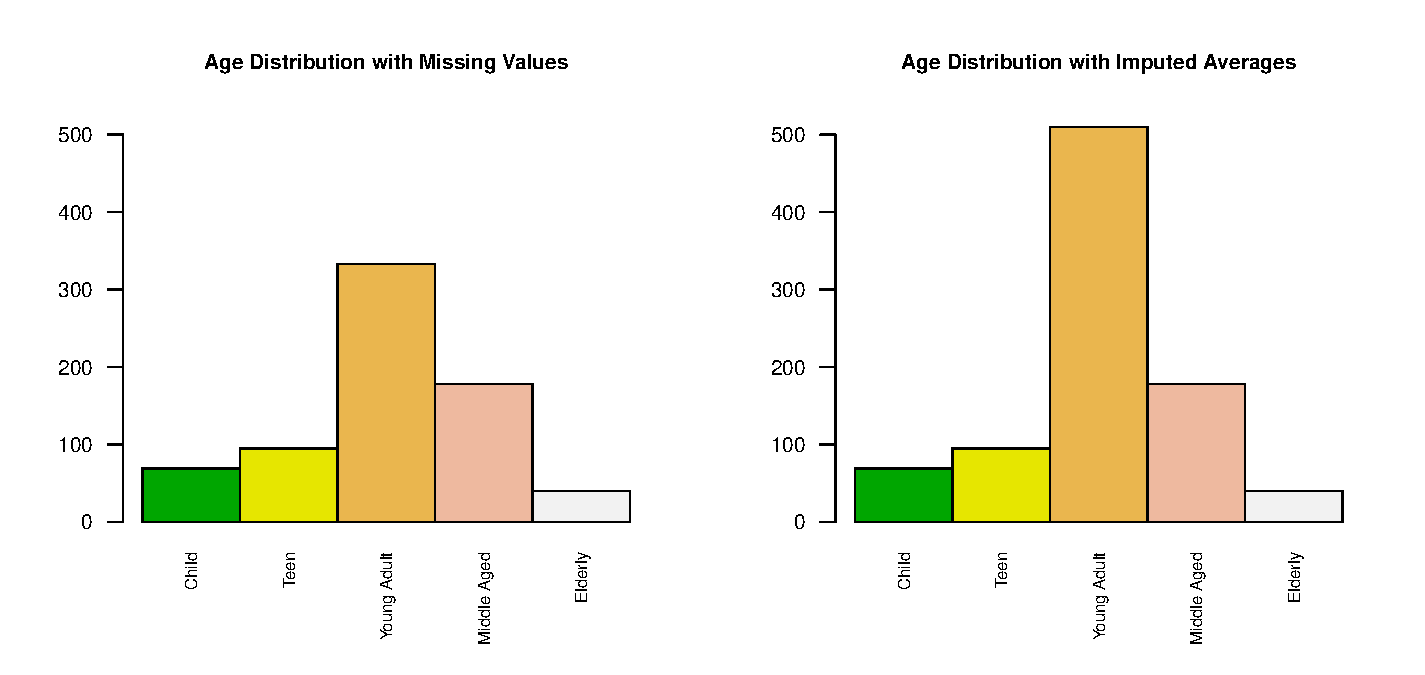
\includegraphics{Titanic_Survival_files/figure-latex/unnamed-chunk-21-1.pdf}

Notice how numerical attributes (\texttt{Age} and \texttt{Fare}) combine
well into a scatterplot, yet other attributes are not plotted exactly as
we might want. Since the problem space will only increase with
higher-dimensional combinations, we select only a few choice pairs to
consider. One approach is to compare each of the other ten features with
our \texttt{Survived} outcome.

\subsection{Interactions with
Survival}\label{interactions-with-survival}

\begin{itemize}
\tightlist
\item
  1 Survived \& Pclass
\end{itemize}

A mosaic plot shows neatly this interaction:

\begin{Shaded}
\begin{Highlighting}[]
\CommentTok{# 1. Survived and Pclass }
\KeywordTok{suppressMessages}\NormalTok{(}\KeywordTok{require}\NormalTok{(ggplot2))}
\KeywordTok{suppressMessages}\NormalTok{(}\KeywordTok{require}\NormalTok{(ggmosaic))}
\end{Highlighting}
\end{Shaded}

\begin{verbatim}
## Warning: package 'ggmosaic' was built under R version 3.5.3
\end{verbatim}

\begin{Shaded}
\begin{Highlighting}[]
\NormalTok{Survival <-}\StringTok{ }\KeywordTok{ifelse}\NormalTok{(train}\OperatorTok{$}\NormalTok{SurvivedNum}\OperatorTok{==}\DecValTok{1}\NormalTok{,}\StringTok{"yes"}\NormalTok{,}\StringTok{"no"}\NormalTok{) }\CommentTok{# for ggplot}
\NormalTok{PclassFac <-}\StringTok{ }\KeywordTok{factor}\NormalTok{(train}\OperatorTok{$}\NormalTok{Pclass)}
\KeywordTok{ggplot}\NormalTok{(}\DataTypeTok{data=}\NormalTok{train) }\OperatorTok{+}
\StringTok{   }\KeywordTok{geom_mosaic}\NormalTok{(}\KeywordTok{aes}\NormalTok{(}\DataTypeTok{x=}\KeywordTok{product}\NormalTok{(Survival, PclassFac),}\DataTypeTok{fill=}\NormalTok{Survival)) }\OperatorTok{+}
\StringTok{   }\KeywordTok{labs}\NormalTok{(}\DataTypeTok{x=}\StringTok{'Passenger Class'}\NormalTok{, }\DataTypeTok{y=}\StringTok{''}\NormalTok{, }\DataTypeTok{title=}\StringTok{'Tianic Survival by Passenger Class'}\NormalTok{)}
\end{Highlighting}
\end{Shaded}

\includegraphics{Titanic_Survival_files/figure-latex/unnamed-chunk-22-1.pdf}

It would seem that folks in first class and second class had it better
than those in third class. What the mosaic plot shows is also the
comparative size of the populations of these three classes (in our
training sample of course).

\begin{itemize}
\tightlist
\item
  2 Survived \& Sex:
\end{itemize}

\begin{Shaded}
\begin{Highlighting}[]
\KeywordTok{ggplot}\NormalTok{(}\DataTypeTok{data=}\NormalTok{train) }\OperatorTok{+}
\StringTok{   }\KeywordTok{geom_mosaic}\NormalTok{(}\KeywordTok{aes}\NormalTok{(}\DataTypeTok{x=}\KeywordTok{product}\NormalTok{(Survival, Sex),}\DataTypeTok{fill=}\NormalTok{Survival)) }\OperatorTok{+}
\StringTok{   }\KeywordTok{labs}\NormalTok{(}\DataTypeTok{x=}\StringTok{'Sex'}\NormalTok{, }\DataTypeTok{y=}\StringTok{''}\NormalTok{, }\DataTypeTok{title=}\StringTok{'Tianic Survival by Gender'}\NormalTok{)}
\end{Highlighting}
\end{Shaded}

\includegraphics{Titanic_Survival_files/figure-latex/unnamed-chunk-23-1.pdf}

Females were much more likely to survive, and the majority of the
passengers was male.

\begin{itemize}
\tightlist
\item
  3 Survived \& Age
\end{itemize}

\begin{Shaded}
\begin{Highlighting}[]
\KeywordTok{plot}\NormalTok{(train}\OperatorTok{$}\NormalTok{SurvivedNum}\OperatorTok{~}\NormalTok{train}\OperatorTok{$}\NormalTok{Age, }\DataTypeTok{pch=}\DecValTok{19}\NormalTok{, }\DataTypeTok{col=}\KeywordTok{rgb}\NormalTok{(}\DecValTok{0}\NormalTok{,}\DecValTok{0}\NormalTok{,.}\DecValTok{6}\NormalTok{,.}\DecValTok{2}\NormalTok{),}
    \DataTypeTok{main=}\StringTok{"Titanic Survival by Age"}\NormalTok{,}\DataTypeTok{ylab=}\StringTok{"Probability of Survival"}\NormalTok{, }\DataTypeTok{xlab=}\StringTok{"Age"}\NormalTok{)}
\NormalTok{linmod=}\KeywordTok{lm}\NormalTok{(SurvivedNum}\OperatorTok{~}\NormalTok{Age,}\DataTypeTok{data=}\NormalTok{train)}
\KeywordTok{abline}\NormalTok{(linmod, }\DataTypeTok{col=}\StringTok{"green"}\NormalTok{, }\DataTypeTok{lwd=}\DecValTok{2}\NormalTok{, }\DataTypeTok{lty=}\DecValTok{2}\NormalTok{)}
\NormalTok{g=}\KeywordTok{glm}\NormalTok{(SurvivedNum}\OperatorTok{~}\NormalTok{Age,}\DataTypeTok{family=}\StringTok{'binomial'}\NormalTok{,}\DataTypeTok{data=}\NormalTok{train)}
\KeywordTok{curve}\NormalTok{(}\KeywordTok{predict}\NormalTok{(g,}\KeywordTok{data.frame}\NormalTok{(}\DataTypeTok{Age=}\NormalTok{x),}\DataTypeTok{type=}\StringTok{"resp"}\NormalTok{),}\DataTypeTok{col=}\StringTok{"red"}\NormalTok{,}\DataTypeTok{lty=}\DecValTok{2}\NormalTok{,}\DataTypeTok{lwd=}\DecValTok{2}\NormalTok{,}\DataTypeTok{add=}\OtherTok{TRUE}\NormalTok{) }
\KeywordTok{legend}\NormalTok{(}\DecValTok{60}\NormalTok{,}\FloatTok{0.7}\NormalTok{,}\KeywordTok{c}\NormalTok{(}\StringTok{"linear fit"}\NormalTok{,}\StringTok{"logistic fit"}\NormalTok{), }\DataTypeTok{col=}\KeywordTok{c}\NormalTok{(}\StringTok{"green"}\NormalTok{,}\StringTok{"red"}\NormalTok{), }\DataTypeTok{lty=}\KeywordTok{c}\NormalTok{(}\DecValTok{1}\NormalTok{,}\DecValTok{2}\NormalTok{))}
\end{Highlighting}
\end{Shaded}

\includegraphics{Titanic_Survival_files/figure-latex/unnamed-chunk-24-1.pdf}

As expected, the probability of survival declines with age, as shown by
the linear fit, which is quite similar to the logistic fit (a sinusoidal
curve) as survival is not rare and the distribution of ages is roughly
normal (as we noted in the univariate EDA), so we observe mid-range
probabilities.

\begin{itemize}
\tightlist
\item
  4 Survived \& SibSp
\end{itemize}

\begin{Shaded}
\begin{Highlighting}[]
\KeywordTok{ggplot}\NormalTok{(}\DataTypeTok{data=}\NormalTok{train) }\OperatorTok{+}
\StringTok{   }\KeywordTok{geom_mosaic}\NormalTok{(}\KeywordTok{aes}\NormalTok{(}\DataTypeTok{x=}\KeywordTok{product}\NormalTok{(Survival, SibSp),}\DataTypeTok{fill=}\NormalTok{Survival)) }\OperatorTok{+}
\StringTok{   }\KeywordTok{labs}\NormalTok{(}\DataTypeTok{x=}\StringTok{'Number of Siblings/Spouses'}\NormalTok{, }\DataTypeTok{y=}\StringTok{''}\NormalTok{, }
   \DataTypeTok{title=}\StringTok{'Tianic Survival by Number of Siblings or Spouses'}\NormalTok{)}
\end{Highlighting}
\end{Shaded}

\includegraphics{Titanic_Survival_files/figure-latex/unnamed-chunk-25-1.pdf}

Having one sibling or spouse is most indicative of survival, followed by
two, then none, then four and up. The probability of survival is very
low for higher numbers but our confidence that this is the case should
decrease because there is gradually less evidence for this effect, given
the smaller sample sizes as shown in the mosaic plot.

\begin{itemize}
\tightlist
\item
  5 Survived \& Parch
\end{itemize}

\begin{Shaded}
\begin{Highlighting}[]
\KeywordTok{ggplot}\NormalTok{(}\DataTypeTok{data=}\NormalTok{train) }\OperatorTok{+}
\StringTok{   }\KeywordTok{geom_mosaic}\NormalTok{(}\KeywordTok{aes}\NormalTok{(}\DataTypeTok{x=}\KeywordTok{product}\NormalTok{(Survival, Parch),}\DataTypeTok{fill=}\NormalTok{Survival)) }\OperatorTok{+}
\StringTok{   }\KeywordTok{labs}\NormalTok{(}\DataTypeTok{x=}\StringTok{'Number of Parents/Children'}\NormalTok{, }\DataTypeTok{y=}\StringTok{''}\NormalTok{, }
   \DataTypeTok{title=}\StringTok{'Tianic Survival by Number of Parents or Children'}\NormalTok{)}
\end{Highlighting}
\end{Shaded}

\includegraphics{Titanic_Survival_files/figure-latex/unnamed-chunk-26-1.pdf}

Similar results to those observed in the previous plot are seen, except
for the higher probability of survival for someone with 3 (presumably)
children, yet again, since the sample sizes are small, we should not
take this finding too seriously.

When \textbf{feature engineering} we will take into account these
findings to select the best method to create our indicator variables.

\begin{itemize}
\tightlist
\item
  6 Survived \& Fare
\end{itemize}

\begin{Shaded}
\begin{Highlighting}[]
\KeywordTok{plot}\NormalTok{(train}\OperatorTok{$}\NormalTok{SurvivedNum}\OperatorTok{~}\NormalTok{train}\OperatorTok{$}\NormalTok{Fare, }\DataTypeTok{pch=}\DecValTok{19}\NormalTok{, }\DataTypeTok{col=}\KeywordTok{rgb}\NormalTok{(}\DecValTok{0}\NormalTok{,}\DecValTok{0}\NormalTok{,.}\DecValTok{6}\NormalTok{,.}\DecValTok{2}\NormalTok{),}
    \DataTypeTok{main=}\StringTok{"Titanic Survival by Fare"}\NormalTok{,}\DataTypeTok{ylab=}\StringTok{"Probability of Survival"}\NormalTok{, }\DataTypeTok{xlab=}\StringTok{"Fare (Pounds Sterling)"}\NormalTok{)}
\NormalTok{linmod=}\KeywordTok{lm}\NormalTok{(SurvivedNum}\OperatorTok{~}\NormalTok{Fare,}\DataTypeTok{data=}\NormalTok{train)}
\KeywordTok{abline}\NormalTok{(linmod, }\DataTypeTok{col=}\StringTok{"green"}\NormalTok{, }\DataTypeTok{lwd=}\DecValTok{1}\NormalTok{, }\DataTypeTok{lty=}\DecValTok{2}\NormalTok{)}
\NormalTok{g=}\KeywordTok{glm}\NormalTok{(SurvivedNum}\OperatorTok{~}\NormalTok{Fare,}\DataTypeTok{family=}\StringTok{'binomial'}\NormalTok{,}\DataTypeTok{data=}\NormalTok{train)}
\KeywordTok{curve}\NormalTok{(}\KeywordTok{predict}\NormalTok{(g,}\KeywordTok{data.frame}\NormalTok{(}\DataTypeTok{Fare=}\NormalTok{x),}\DataTypeTok{type=}\StringTok{"resp"}\NormalTok{),}\DataTypeTok{col=}\StringTok{"red"}\NormalTok{,}\DataTypeTok{lty=}\DecValTok{2}\NormalTok{,}\DataTypeTok{lwd=}\DecValTok{2}\NormalTok{,}\DataTypeTok{add=}\OtherTok{TRUE}\NormalTok{) }
\KeywordTok{legend}\NormalTok{(}\DecValTok{200}\NormalTok{,}\FloatTok{0.7}\NormalTok{,}\KeywordTok{c}\NormalTok{(}\StringTok{"linear fit"}\NormalTok{,}\StringTok{"logistic fit"}\NormalTok{), }\DataTypeTok{col=}\KeywordTok{c}\NormalTok{(}\StringTok{"green"}\NormalTok{,}\StringTok{"red"}\NormalTok{), }\DataTypeTok{lty=}\KeywordTok{c}\NormalTok{(}\DecValTok{1}\NormalTok{,}\DecValTok{2}\NormalTok{))}
\end{Highlighting}
\end{Shaded}

\includegraphics{Titanic_Survival_files/figure-latex/unnamed-chunk-27-1.pdf}

Unlike the plot of Survival by Age, we observe extreme probabilities
given the skewed distribution of Fare, which shows how survival is
increasingly more probable the higher the fare.

We can explore creating a log of Fare which could be used in modeling,
as some models (i.e.~linear models) would benefit from this logged
variable as opposed to the original Fare attribute.

\begin{Shaded}
\begin{Highlighting}[]
\CommentTok{# creating Log of Fare attribute}
\NormalTok{train}\OperatorTok{$}\NormalTok{FareLog <-}\StringTok{ }\KeywordTok{log}\NormalTok{(train}\OperatorTok{$}\NormalTok{Fare}\OperatorTok{+}\DecValTok{1}\NormalTok{) }\CommentTok{# adding a pound to avoid Inf log values for 0 fares}
\CommentTok{# plot}
\KeywordTok{plot}\NormalTok{(train}\OperatorTok{$}\NormalTok{SurvivedNum}\OperatorTok{~}\NormalTok{train}\OperatorTok{$}\NormalTok{FareLog, }\DataTypeTok{pch=}\DecValTok{19}\NormalTok{, }\DataTypeTok{col=}\KeywordTok{rgb}\NormalTok{(}\DecValTok{0}\NormalTok{,}\DecValTok{0}\NormalTok{,.}\DecValTok{6}\NormalTok{,.}\DecValTok{2}\NormalTok{),}
    \DataTypeTok{main=}\StringTok{"Titanic Survival by Log of Fare"}\NormalTok{,}
    \DataTypeTok{ylab=}\StringTok{"Probability of Survival"}\NormalTok{, }\DataTypeTok{xlab=}\StringTok{"Fare in Log(Pounds Sterling)"}\NormalTok{)}
\NormalTok{linmod=}\KeywordTok{lm}\NormalTok{(SurvivedNum}\OperatorTok{~}\NormalTok{FareLog,}\DataTypeTok{data=}\NormalTok{train)}
\KeywordTok{abline}\NormalTok{(linmod, }\DataTypeTok{col=}\StringTok{"green"}\NormalTok{, }\DataTypeTok{lwd=}\DecValTok{1}\NormalTok{, }\DataTypeTok{lty=}\DecValTok{2}\NormalTok{)}
\NormalTok{g=}\KeywordTok{glm}\NormalTok{(SurvivedNum}\OperatorTok{~}\NormalTok{FareLog,}\DataTypeTok{family=}\StringTok{'binomial'}\NormalTok{,}\DataTypeTok{data=}\NormalTok{train)}
\KeywordTok{curve}\NormalTok{(}\KeywordTok{predict}\NormalTok{(g,}\KeywordTok{data.frame}\NormalTok{(}\DataTypeTok{FareLog=}\NormalTok{x),}\DataTypeTok{type=}\StringTok{"resp"}\NormalTok{),}\DataTypeTok{col=}\StringTok{"red"}\NormalTok{,}\DataTypeTok{lty=}\DecValTok{2}\NormalTok{,}\DataTypeTok{lwd=}\DecValTok{2}\NormalTok{,}\DataTypeTok{add=}\OtherTok{TRUE}\NormalTok{) }
\KeywordTok{legend}\NormalTok{(}\DecValTok{1}\NormalTok{,}\FloatTok{0.7}\NormalTok{,}\KeywordTok{c}\NormalTok{(}\StringTok{"linear fit"}\NormalTok{,}\StringTok{"logistic fit"}\NormalTok{), }\DataTypeTok{col=}\KeywordTok{c}\NormalTok{(}\StringTok{"green"}\NormalTok{,}\StringTok{"red"}\NormalTok{), }\DataTypeTok{lty=}\KeywordTok{c}\NormalTok{(}\DecValTok{1}\NormalTok{,}\DecValTok{2}\NormalTok{))}
\end{Highlighting}
\end{Shaded}

\includegraphics{Titanic_Survival_files/figure-latex/unnamed-chunk-28-1.pdf}

The \texttt{FareLog} variable will indeed be useful for linear modeling.

\begin{itemize}
\tightlist
\item
  7 Survived \& Cabin
\end{itemize}

Since our data has so many missing values for cabin, our confidence in
the results of this plot should be decreased.

\begin{Shaded}
\begin{Highlighting}[]
\CommentTok{# creating a copy of train with no missing values for cabin}
\NormalTok{train2 <-}\StringTok{ }\NormalTok{train[}\OperatorTok{!}\KeywordTok{is.na}\NormalTok{(train}\OperatorTok{$}\NormalTok{Cabin),]}
\NormalTok{Survival2 <-}\StringTok{ }\KeywordTok{ifelse}\NormalTok{(train2}\OperatorTok{$}\NormalTok{SurvivedNum}\OperatorTok{==}\DecValTok{1}\NormalTok{,}\StringTok{"yes"}\NormalTok{,}\StringTok{"no"}\NormalTok{) }
\KeywordTok{ggplot}\NormalTok{(}\DataTypeTok{data=}\NormalTok{train2) }\OperatorTok{+}
\StringTok{   }\KeywordTok{geom_mosaic}\NormalTok{(}\KeywordTok{aes}\NormalTok{(}\DataTypeTok{x=}\KeywordTok{product}\NormalTok{(Survival2, Cabin),}\DataTypeTok{fill=}\NormalTok{Survival2)) }\OperatorTok{+}
\StringTok{   }\KeywordTok{labs}\NormalTok{(}\DataTypeTok{x=}\StringTok{'Cabin'}\NormalTok{, }\DataTypeTok{y=}\StringTok{''}\NormalTok{, }\DataTypeTok{title=}\StringTok{'Tianic Survival by Cabin'}\NormalTok{)}
\end{Highlighting}
\end{Shaded}

\includegraphics{Titanic_Survival_files/figure-latex/unnamed-chunk-29-1.pdf}

It would appear that perhaps cabin is not as associated with
survivability as we had hoped for, given that A cabins are on the deck
and F cabins near the keel where the ship hit the iceberg.

\begin{itemize}
\tightlist
\item
  8 Survived \& Embarked
\end{itemize}

\begin{Shaded}
\begin{Highlighting}[]
\NormalTok{PortEmbarked <-}\StringTok{ }\KeywordTok{ifelse}\NormalTok{(train}\OperatorTok{$}\NormalTok{Embarked}\OperatorTok{==}\StringTok{"C"}\NormalTok{,}\StringTok{"Cherbourg"}\NormalTok{, }
                \KeywordTok{ifelse}\NormalTok{(train}\OperatorTok{$}\NormalTok{Embarked}\OperatorTok{==}\StringTok{"Q"}\NormalTok{,}\StringTok{"Queenstown"}\NormalTok{, }\StringTok{"Southampton"}\NormalTok{))}
\NormalTok{dat <-}\StringTok{ }\KeywordTok{data.frame}\NormalTok{(Survival, PortEmbarked)}

\KeywordTok{ggplot}\NormalTok{(}\DataTypeTok{data=}\NormalTok{dat) }\OperatorTok{+}
\StringTok{   }\KeywordTok{geom_mosaic}\NormalTok{(}\KeywordTok{aes}\NormalTok{(}\DataTypeTok{x=}\KeywordTok{product}\NormalTok{(Survival, PortEmbarked),}\DataTypeTok{fill=}\NormalTok{Survival)) }\OperatorTok{+}
\StringTok{   }\KeywordTok{labs}\NormalTok{(}\DataTypeTok{x=}\StringTok{'Port of Embarkation'}\NormalTok{, }\DataTypeTok{y=}\StringTok{''}\NormalTok{, }
   \DataTypeTok{title=}\StringTok{'Tianic Survival by Port of Embarkation'}\NormalTok{)}
\end{Highlighting}
\end{Shaded}

\includegraphics{Titanic_Survival_files/figure-latex/unnamed-chunk-30-1.pdf}

There seems to be some evidence that having embarked in Southhampton is
an indicator of higher probability of survival.

We can explore port of embarkation in a more nuanced manner by
considering the fares paid at each port, and whether survivability
appears to me more associated with the fare or the port embarked. We use
the log of fares since it would be hard to observe any differences in
the boxplots given the highly skewed distribution of fare.

\begin{Shaded}
\begin{Highlighting}[]
\NormalTok{dat}\OperatorTok{$}\NormalTok{FareLog <-}\StringTok{ }\NormalTok{train}\OperatorTok{$}\NormalTok{FareLog}
\NormalTok{dat <-}\StringTok{ }\NormalTok{dat[}\OperatorTok{!}\KeywordTok{is.na}\NormalTok{(dat}\OperatorTok{$}\NormalTok{PortEmbarked),]}
\KeywordTok{ggplot}\NormalTok{(}\DataTypeTok{data=}\NormalTok{dat) }\OperatorTok{+}
\StringTok{   }\KeywordTok{geom_boxplot}\NormalTok{(}\KeywordTok{aes}\NormalTok{(}\DataTypeTok{x=}\NormalTok{PortEmbarked,}\DataTypeTok{y=}\NormalTok{FareLog, }\DataTypeTok{fill=}\NormalTok{Survival)) }\OperatorTok{+}
\StringTok{   }\KeywordTok{labs}\NormalTok{(}\DataTypeTok{x=}\StringTok{'Port of Embarkation'}\NormalTok{, }\DataTypeTok{y=}\StringTok{'Fare in Log(Pounds Sterling)'}\NormalTok{, }
   \DataTypeTok{title=}\StringTok{'Titanic Survival by Port of Embarkation and Fare'}\NormalTok{)}
\end{Highlighting}
\end{Shaded}

\includegraphics{Titanic_Survival_files/figure-latex/unnamed-chunk-31-1.pdf}

Several curiosities pop out in this plot. First, Southhampton's higher
survivability is not entirely associated with fare, since Cherbourg
seems to have a higher survivability when considering fare. Second,
Queenstown's seems to go against common sense in that higher fares
aren't necessarily associated with higher survivability. Lastly, the
difference in survivability according to fare varies from port to port,
for example, we see a more pronounced difference in Cherbourg, and
almost no difference in Queenstown.

\begin{itemize}
\tightlist
\item
  9 Survival and Title
\end{itemize}

\begin{Shaded}
\begin{Highlighting}[]
\KeywordTok{ggplot}\NormalTok{(}\DataTypeTok{data=}\NormalTok{train) }\OperatorTok{+}
\StringTok{   }\KeywordTok{geom_mosaic}\NormalTok{(}\KeywordTok{aes}\NormalTok{(}\DataTypeTok{x=}\KeywordTok{product}\NormalTok{(Survival, Title),}\DataTypeTok{fill=}\NormalTok{Survival)) }\OperatorTok{+}\StringTok{ }
\StringTok{   }\KeywordTok{labs}\NormalTok{(}\DataTypeTok{x=}\StringTok{'Title'}\NormalTok{, }\DataTypeTok{y=}\StringTok{''}\NormalTok{,}
   \DataTypeTok{title=}\StringTok{'Tianic Survival by Title'}\NormalTok{) }\OperatorTok{+}\StringTok{ }
\StringTok{   }\KeywordTok{theme}\NormalTok{(}\DataTypeTok{axis.text.x =} \KeywordTok{element_text}\NormalTok{(}\DataTypeTok{angle =} \DecValTok{90}\NormalTok{))}
\end{Highlighting}
\end{Shaded}

\includegraphics{Titanic_Survival_files/figure-latex/unnamed-chunk-32-1.pdf}

Title can be seen as a proxy for gender and as we've seen, females
survived a lot better than males. It is worth keeping this attribute as
it shows some granularity in what kinds of folks survived better within
gender groups, i.e.~those with rare titles.

\begin{itemize}
\item
  \begin{enumerate}
  \def\labelenumi{\arabic{enumi}.}
  \setcounter{enumi}{9}
  \tightlist
  \item
    Survived and NameLength
  \end{enumerate}
\end{itemize}

\begin{Shaded}
\begin{Highlighting}[]
\KeywordTok{plot}\NormalTok{(train}\OperatorTok{$}\NormalTok{SurvivedNum}\OperatorTok{~}\NormalTok{train}\OperatorTok{$}\NormalTok{NameLength, }\DataTypeTok{pch=}\DecValTok{19}\NormalTok{, }\DataTypeTok{col=}\KeywordTok{rgb}\NormalTok{(}\DecValTok{0}\NormalTok{,}\DecValTok{0}\NormalTok{,.}\DecValTok{6}\NormalTok{,.}\DecValTok{2}\NormalTok{),}
    \DataTypeTok{main=}\StringTok{"Titanic Survival by Name Length"}\NormalTok{,}
    \DataTypeTok{ylab=}\StringTok{"Probability of Survival"}\NormalTok{, }\DataTypeTok{xlab=}\StringTok{"Name Length (chars)"}\NormalTok{)}
\NormalTok{linmod=}\KeywordTok{lm}\NormalTok{(SurvivedNum}\OperatorTok{~}\NormalTok{NameLength,}\DataTypeTok{data=}\NormalTok{train)}
\KeywordTok{abline}\NormalTok{(linmod, }\DataTypeTok{col=}\StringTok{"green"}\NormalTok{, }\DataTypeTok{lwd=}\DecValTok{1}\NormalTok{, }\DataTypeTok{lty=}\DecValTok{2}\NormalTok{)}
\NormalTok{g=}\KeywordTok{glm}\NormalTok{(SurvivedNum}\OperatorTok{~}\NormalTok{NameLength,}\DataTypeTok{family=}\StringTok{'binomial'}\NormalTok{,}\DataTypeTok{data=}\NormalTok{train)}
\KeywordTok{curve}\NormalTok{(}\KeywordTok{predict}\NormalTok{(g,}\KeywordTok{data.frame}\NormalTok{(}\DataTypeTok{NameLength=}\NormalTok{x),}\DataTypeTok{type=}\StringTok{"resp"}\NormalTok{),}\DataTypeTok{col=}\StringTok{"red"}\NormalTok{,}\DataTypeTok{lty=}\DecValTok{2}\NormalTok{,}\DataTypeTok{lwd=}\DecValTok{2}\NormalTok{,}\DataTypeTok{add=}\OtherTok{TRUE}\NormalTok{) }
\KeywordTok{legend}\NormalTok{(}\DecValTok{60}\NormalTok{,}\FloatTok{0.5}\NormalTok{,}\KeywordTok{c}\NormalTok{(}\StringTok{"linear fit"}\NormalTok{,}\StringTok{"logistic fit"}\NormalTok{), }\DataTypeTok{col=}\KeywordTok{c}\NormalTok{(}\StringTok{"green"}\NormalTok{,}\StringTok{"red"}\NormalTok{), }\DataTypeTok{lty=}\KeywordTok{c}\NormalTok{(}\DecValTok{1}\NormalTok{,}\DecValTok{2}\NormalTok{))}
\end{Highlighting}
\end{Shaded}

\includegraphics{Titanic_Survival_files/figure-latex/unnamed-chunk-33-1.pdf}

Longer names do appear to have some association with higher
probabilities of survival so we are also keeping this feature. It might
just be capturing the association of longer names and wealth, but since
in machine learning we do not care about multicollinearity issues, we
will test whether to keep this attribute or not during our feature
selection modeling phase.

\begin{center}\rule{0.5\linewidth}{\linethickness}\end{center}

\subsection{Multi-dimensional EDA}\label{multi-dimensional-eda}

The higher-dimensional problem space of combinations with 11 variables
is as follows:

\begin{Shaded}
\begin{Highlighting}[]
\CommentTok{# Combinations of 3 or more variables quickly explode}
\NormalTok{vars <-}\StringTok{ }\DecValTok{1}\OperatorTok{:}\DecValTok{11}
\ControlFlowTok{for}\NormalTok{ (i }\ControlFlowTok{in} \DecValTok{2}\OperatorTok{:}\DecValTok{9}\NormalTok{) \{}
\NormalTok{    num <-}\StringTok{ }\KeywordTok{length}\NormalTok{(}\KeywordTok{combn}\NormalTok{(vars,i))}\OperatorTok{/}\NormalTok{i}
    \KeywordTok{print}\NormalTok{(}\KeywordTok{paste}\NormalTok{(}\StringTok{"There are "}\NormalTok{, num, }\StringTok{"combinations of 11 variables taken"}\NormalTok{, i, }\StringTok{"at a time."}\NormalTok{))}
\NormalTok{\}}
\end{Highlighting}
\end{Shaded}

\begin{verbatim}
## [1] "There are  55 combinations of 11 variables taken 2 at a time."
## [1] "There are  165 combinations of 11 variables taken 3 at a time."
## [1] "There are  330 combinations of 11 variables taken 4 at a time."
## [1] "There are  462 combinations of 11 variables taken 5 at a time."
## [1] "There are  462 combinations of 11 variables taken 6 at a time."
## [1] "There are  330 combinations of 11 variables taken 7 at a time."
## [1] "There are  165 combinations of 11 variables taken 8 at a time."
## [1] "There are  55 combinations of 11 variables taken 9 at a time."
\end{verbatim}

The number of combinations is complementary (adding up to 11): 6 = 5, 7
= 4, etc., so when considering combinations of 9 variables, we are just
considering the complement of 2 variables.

Of the 165 trivariate combinations, 45 alone are possibilities that
interact with our outcome \texttt{Survival} -- clearly too many to
consider, so our approach will by means of necessity be minimal and
select, but I wanted to make the size of the entire enterprise known.

\subsection{Age Categories and
Imputation}\label{age-categories-and-imputation}

To make matters worse, I am breaking down the \texttt{Age} continuous
variable into four new features by age group: \texttt{Child} (\(0-12\))
\texttt{Teen} (\(13-19\)), \texttt{YoungAdult} (\(20-35\)),
\texttt{MiddleAged} (\(36-55\)), and \texttt{Elderly} (\(56-80\)). While
some of these age groups might seem young by 2019's standards, at the
time of the Titanic's maiden voyage, I believe they more accurately
reflect the respective age groups, as evidenced by the distribution
below. This breakdown will help later with machine learning but also
help EDA in exploring age groups in a discrete manner.

Before we actually create these features, however, we need to impute the
missing values. One strategy is to use a mean or median age, which would
unnecessarily inflate the \texttt{YoungAdult} variable, as seen in the
second plot below.

\begin{Shaded}
\begin{Highlighting}[]
\NormalTok{Child <-}\StringTok{ }\KeywordTok{sum}\NormalTok{(}\KeywordTok{ifelse}\NormalTok{(train}\OperatorTok{$}\NormalTok{Age }\OperatorTok{>}\StringTok{ }\DecValTok{0} \OperatorTok{&}\StringTok{ }\NormalTok{train}\OperatorTok{$}\NormalTok{Age }\OperatorTok{<}\StringTok{ }\DecValTok{13}\NormalTok{,}\DecValTok{1}\NormalTok{,}\DecValTok{0}\NormalTok{),}\DataTypeTok{na.rm=}\OtherTok{TRUE}\NormalTok{)}
\NormalTok{Teen <-}\StringTok{  }\KeywordTok{sum}\NormalTok{(}\KeywordTok{ifelse}\NormalTok{(train}\OperatorTok{$}\NormalTok{Age }\OperatorTok{>}\StringTok{ }\DecValTok{12} \OperatorTok{&}\StringTok{ }\NormalTok{train}\OperatorTok{$}\NormalTok{Age }\OperatorTok{<}\StringTok{ }\DecValTok{20}\NormalTok{,}\DecValTok{1}\NormalTok{,}\DecValTok{0}\NormalTok{),}\DataTypeTok{na.rm=}\OtherTok{TRUE}\NormalTok{)}
\NormalTok{YoungAdult <-}\StringTok{ }\KeywordTok{sum}\NormalTok{(}\KeywordTok{ifelse}\NormalTok{(train}\OperatorTok{$}\NormalTok{Age }\OperatorTok{>}\StringTok{ }\DecValTok{19} \OperatorTok{&}\StringTok{ }\NormalTok{train}\OperatorTok{$}\NormalTok{Age }\OperatorTok{<}\StringTok{ }\DecValTok{36}\NormalTok{,}\DecValTok{1}\NormalTok{,}\DecValTok{0}\NormalTok{),}\DataTypeTok{na.rm=}\OtherTok{TRUE}\NormalTok{)}
\NormalTok{MiddleAged <-}\StringTok{ }\KeywordTok{sum}\NormalTok{(}\KeywordTok{ifelse}\NormalTok{(train}\OperatorTok{$}\NormalTok{Age }\OperatorTok{>}\StringTok{ }\DecValTok{35} \OperatorTok{&}\StringTok{ }\NormalTok{train}\OperatorTok{$}\NormalTok{Age }\OperatorTok{<}\StringTok{ }\DecValTok{56}\NormalTok{,}\DecValTok{1}\NormalTok{,}\DecValTok{0}\NormalTok{),}\DataTypeTok{na.rm=}\OtherTok{TRUE}\NormalTok{)}
\NormalTok{Elderly <-}\StringTok{ }\KeywordTok{sum}\NormalTok{(}\KeywordTok{ifelse}\NormalTok{(train}\OperatorTok{$}\NormalTok{Age }\OperatorTok{>}\StringTok{ }\DecValTok{55} \OperatorTok{&}\StringTok{ }\NormalTok{train}\OperatorTok{$}\NormalTok{Age }\OperatorTok{<}\StringTok{ }\DecValTok{100}\NormalTok{,}\DecValTok{1}\NormalTok{,}\DecValTok{0}\NormalTok{),}\DataTypeTok{na.rm=}\OtherTok{TRUE}\NormalTok{)}
\NormalTok{vec <-}\StringTok{ }\KeywordTok{c}\NormalTok{(Child,Teen,YoungAdult,MiddleAged,Elderly)}
\KeywordTok{par}\NormalTok{(}\DataTypeTok{mfrow=}\KeywordTok{c}\NormalTok{(}\DecValTok{1}\NormalTok{,}\DecValTok{2}\NormalTok{))}
\KeywordTok{barplot}\NormalTok{(vec, }\DataTypeTok{col=}\KeywordTok{terrain.colors}\NormalTok{(}\DecValTok{5}\NormalTok{), }\DataTypeTok{ylim=}\KeywordTok{c}\NormalTok{(}\DecValTok{0}\NormalTok{,}\DecValTok{515}\NormalTok{),}
        \DataTypeTok{cex.names=}\NormalTok{.}\DecValTok{7}\NormalTok{, }\DataTypeTok{cex.main=}\FloatTok{0.8}\NormalTok{, }\DataTypeTok{cex.axis=}\FloatTok{0.8}\NormalTok{, }\DataTypeTok{las=}\DecValTok{2}\NormalTok{,}
        \DataTypeTok{main=}\StringTok{"Age Distribution with Missing Values"}\NormalTok{,  }\DataTypeTok{space=}\KeywordTok{c}\NormalTok{(}\DecValTok{0}\NormalTok{,}\DecValTok{0}\NormalTok{,}\DecValTok{0}\NormalTok{,}\DecValTok{0}\NormalTok{,}\DecValTok{0}\NormalTok{),}
        \DataTypeTok{names.arg=}\KeywordTok{c}\NormalTok{(}\StringTok{"Child"}\NormalTok{,}\StringTok{"Teen"}\NormalTok{,}\StringTok{"Young Adult"}\NormalTok{,}\StringTok{"Middle Aged"}\NormalTok{,}\StringTok{"Elderly"}\NormalTok{))}
\CommentTok{# adding all 177 NAs to the Young Adult category}
\NormalTok{YoungAdult <-}\StringTok{ }\NormalTok{YoungAdult }\OperatorTok{+}\StringTok{ }\KeywordTok{sum}\NormalTok{(}\KeywordTok{is.na}\NormalTok{(train}\OperatorTok{$}\NormalTok{Age))}
\NormalTok{vec <-}\StringTok{ }\KeywordTok{c}\NormalTok{(Child,Teen,YoungAdult,MiddleAged,Elderly)}
\KeywordTok{barplot}\NormalTok{(vec, }\DataTypeTok{col=}\KeywordTok{terrain.colors}\NormalTok{(}\DecValTok{5}\NormalTok{), }\DataTypeTok{ylim=}\KeywordTok{c}\NormalTok{(}\DecValTok{0}\NormalTok{,}\DecValTok{515}\NormalTok{),}
        \DataTypeTok{cex.names=}\NormalTok{.}\DecValTok{7}\NormalTok{, }\DataTypeTok{cex.main=}\FloatTok{0.8}\NormalTok{, }\DataTypeTok{cex.axis=}\FloatTok{0.8}\NormalTok{, }\DataTypeTok{las=}\DecValTok{2}\NormalTok{,}
        \DataTypeTok{main=}\StringTok{"Age Distribution with Imputed Averages"}\NormalTok{, }\DataTypeTok{space=}\KeywordTok{c}\NormalTok{(}\DecValTok{0}\NormalTok{,}\DecValTok{0}\NormalTok{,}\DecValTok{0}\NormalTok{,}\DecValTok{0}\NormalTok{,}\DecValTok{0}\NormalTok{),}
        \DataTypeTok{names.arg=}\KeywordTok{c}\NormalTok{(}\StringTok{"Child"}\NormalTok{,}\StringTok{"Teen"}\NormalTok{,}\StringTok{"Young Adult"}\NormalTok{,}\StringTok{"Middle Aged"}\NormalTok{,}\StringTok{"Elderly"}\NormalTok{))}
\end{Highlighting}
\end{Shaded}

\includegraphics{Titanic_Survival_files/figure-latex/unnamed-chunk-35-1.pdf}

Another strategy would be to \textbf{generate random values} given a
similar distribution to that which we observed in our traning data, yet
one problem with this approach is that it overfits the values we
observe, reinforcing patterns that might not necessarily be
generalizable.

A final and more sophisticated approach would be to use the rest of the
information in the training data and \textbf{generate predictions} for
the ages of those individuals, based on other attributes. Since Decision
Tree models are easy to use and accept missing values and unscaled
features and so forth, we can easily generate ages without much hassle
and modeling work.

\begin{Shaded}
\begin{Highlighting}[]
\KeywordTok{library}\NormalTok{(tree)}
\KeywordTok{library}\NormalTok{(caTools)}

\StringTok{'%ni%'}\NormalTok{ <-}\StringTok{ }\KeywordTok{Negate}\NormalTok{(}\StringTok{'%in%'}\NormalTok{)}
\NormalTok{out_vars <-}\StringTok{ }\KeywordTok{c}\NormalTok{(}\StringTok{"SurvivedFac"}\NormalTok{,}\StringTok{"FareLog"}\NormalTok{) }\CommentTok{# we do not need these redundant features}
\NormalTok{Y <-}\StringTok{ }\NormalTok{train[,}\KeywordTok{colnames}\NormalTok{(train)}\OperatorTok{==}\StringTok{"SurvivedNum"}\NormalTok{] }\CommentTok{# outcome }

\KeywordTok{set.seed}\NormalTok{(}\DecValTok{123}\NormalTok{) }\CommentTok{# set random seed for reproducibility}
\NormalTok{tree_bool <-}\StringTok{ }\KeywordTok{sample.split}\NormalTok{(Y, }\DataTypeTok{SplitRatio =} \DecValTok{2}\OperatorTok{/}\DecValTok{3}\NormalTok{) }\CommentTok{# see note below re: proportions}
\NormalTok{tree_train <-}\StringTok{ }\NormalTok{train[tree_bool,}\KeywordTok{colnames}\NormalTok{(train) }\OperatorTok\StringTok{ }\NormalTok{out_vars]}
\NormalTok{tree_test <-}\StringTok{ }\NormalTok{train[}\OperatorTok{!}\NormalTok{tree_bool,}\KeywordTok{colnames}\NormalTok{(train) }\OperatorTok\StringTok{ }\NormalTok{out_vars]}

\CommentTok{# sample.split() performs proportionate sampling of the outcome}
\KeywordTok{table}\NormalTok{(tree_train}\OperatorTok{$}\NormalTok{SurvivedNum)}\OperatorTok{/}\KeywordTok{nrow}\NormalTok{(tree_train)}
\end{Highlighting}
\end{Shaded}

\begin{verbatim}
## 
##         0         1 
## 0.6161616 0.3838384
\end{verbatim}

\begin{Shaded}
\begin{Highlighting}[]
\KeywordTok{table}\NormalTok{(tree_test}\OperatorTok{$}\NormalTok{SurvivedNum)}\OperatorTok{/}\KeywordTok{nrow}\NormalTok{(tree_test)}
\end{Highlighting}
\end{Shaded}

\begin{verbatim}
## 
##         0         1 
## 0.6161616 0.3838384
\end{verbatim}

\begin{Shaded}
\begin{Highlighting}[]
\NormalTok{tree_train_mod <-}\StringTok{ }\KeywordTok{tree}\NormalTok{(SurvivedNum}\OperatorTok{~}\NormalTok{.,}\DataTypeTok{data=}\NormalTok{tree_train)}
\KeywordTok{summary}\NormalTok{(tree_train_mod)}
\end{Highlighting}
\end{Shaded}

\begin{verbatim}
## 
## Regression tree:
## tree(formula = SurvivedNum ~ ., data = tree_train)
## Variables actually used in tree construction:
## [1] "Title" "Cabin" "Age"   "SibSp" "Parch"
## Number of terminal nodes:  12 
## Residual mean deviance:  0.1016 = 11.18 / 110 
## Distribution of residuals:
##     Min.  1st Qu.   Median     Mean  3rd Qu.     Max. 
## -0.97560  0.00000  0.02439  0.00000  0.02439  0.77780
\end{verbatim}

\begin{Shaded}
\begin{Highlighting}[]
\KeywordTok{plot}\NormalTok{(tree_train_mod)}
\KeywordTok{text}\NormalTok{(tree_train_mod, }\DataTypeTok{pretty=}\DecValTok{0}\NormalTok{)}
\end{Highlighting}
\end{Shaded}

\includegraphics{Titanic_Survival_files/figure-latex/unnamed-chunk-38-1.pdf}


\end{document}
